\documentclass{standalone}
\usepackage{pgfplots}
\begin{document}
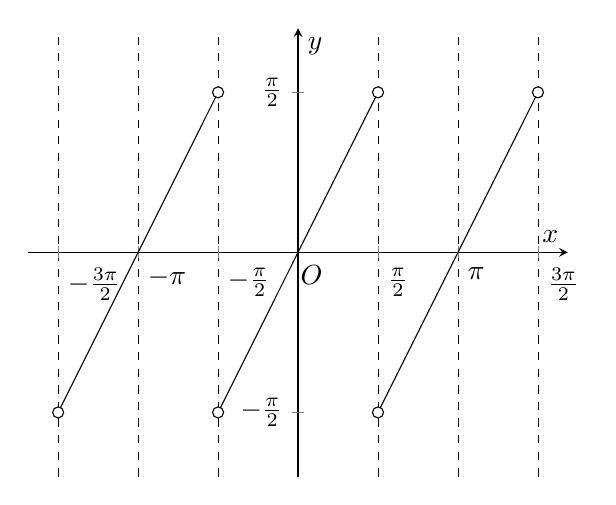
\begin{tikzpicture}
\begin{axis}
[
ymin=-2.2,ymax=2.2,
xmin=-5.3,xmax=5.3,
xtick=\empty,
ytick=\empty,
extra x ticks={-4.71239, -3.14159, -1.5708, 1.5708, 3.14159, 4.71239},
extra x tick labels={$-\frac{3\pi}{2}$, $-\pi$, $-\frac{\pi}{2}$, $\frac{\pi}{2}$, $\pi$, $\frac{3\pi}{2}$},
extra y ticks={-1.5708, 1.5708},
extra y tick labels={$-\frac{\pi}{2}$, $\frac{\pi}{2}$},
every extra x tick/.style={
    xticklabel style={anchor=north west},
    grid=major,
    major grid style={very thin,dashed,black}
},
axis lines = center,
xlabel=$x$,ylabel=$y$,
samples=200,
]
\addplot [black] coordinates {(-4.71239,-1.5708) (-1.5708,1.5708)};
\addplot [black, only marks, mark=*, mark options={fill=white}] coordinates {(-4.71239,-1.5708)};
\addplot [black, only marks, mark=*, mark options={fill=white}] coordinates {(-1.5708,1.5708)};
\addplot [black] coordinates {(-1.5708,-1.5708) (1.5708,1.5708)};
\addplot [black, only marks, mark=*, mark options={fill=white}] coordinates {(-1.5708,-1.5708)};
\addplot [black, only marks, mark=*, mark options={fill=white}] coordinates {(1.5708,1.5708)};
\addplot [black] coordinates {(1.5708,-1.5708) (4.71239,1.5708)};
\addplot [black, only marks, mark=*, mark options={fill=white}] coordinates {(1.5708,-1.5708)};
\addplot [black, only marks, mark=*, mark options={fill=white}] coordinates {(4.71239,1.5708)};
\node at (axis cs:0.265, -0.22) {$O$} ;
\end{axis}
\end{tikzpicture}
\end{document}
